\documentclass[notitlepage]{article}

\usepackage{listings}
\usepackage{color}
\usepackage{graphicx}
\usepackage{float}
\usepackage{fancyhdr}
\usepackage{titlesec}
\pagestyle{fancy}

\usepackage[english]{babel}
\usepackage[utf8]{inputenc}

\pagestyle{fancy}
\fancyhf{}
\rhead{Niklas Vest}
\lhead{\today}
\rfoot{Page \thepage}

\definecolor{dkgreen}{rgb}{0,0.6,0}
\definecolor{gray}{rgb}{0.5,0.5,0.5}
\definecolor{mauve}{rgb}{0.58,0,0.82}

\RequirePackage{ifthen}

\RequirePackage{xcolor}
\definecolor{ListingsBackgroundColor}{gray}{0.95}

\RequirePackage{listingsutf8}
\lstset{
	inputencoding=utf8,
	extendedchars=true,
	basicstyle=\ttfamily\footnotesize,%
	keywordstyle=\color{blue},
	identifierstyle=,%\sffamily, %\bfseries
	commentstyle=\normalfont\itshape\color{brown},%
	stringstyle=\ttfamily\color{purple},%
	showstringspaces=false,%
	columns = flexible,% fixed, 
	breaklines=true,%
	tabsize=2, %
	backgroundcolor=\color{ListingsBackgroundColor},
	xleftmargin=6mm,%
	frame=none,
	framexleftmargin=6mm,
	numbers=left,%
	numbersep=5pt,%
	numberstyle=\normalfont\scriptsize,%
	stepnumber=1,%
	numberfirstline=true,%
	numberblanklines=true,%
	keepspaces=true,%
}

\title{Ausarbeitung 05}
\author{Niklas Vest}
\date{\today}
\begin{document}
	\maketitle
	\thispagestyle{fancy}
	
	\section*{Abfragen}
	\lstinputlisting[language=SQL]{../src/DES33_UE05_VEST.sql}
	\section*{Ergebnisse}
	
	%1.1
	\begin{figure}[H]\centering
		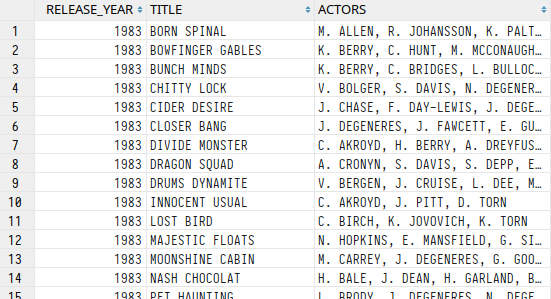
\includegraphics[width=\textwidth]{images/1_1.png}
		\caption{Resultat der Abfrage 1.1}
	\end{figure}

	%1.2
	\begin{figure}[H]\centering
		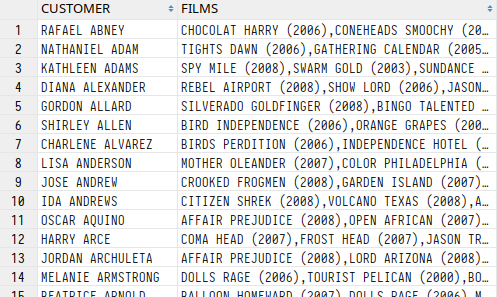
\includegraphics[width=\textwidth]{images/1_2.png}
		\caption{Resultat der Abfrage 1.2}
	\end{figure}

	%1.3
	\begin{figure}[H]\centering
		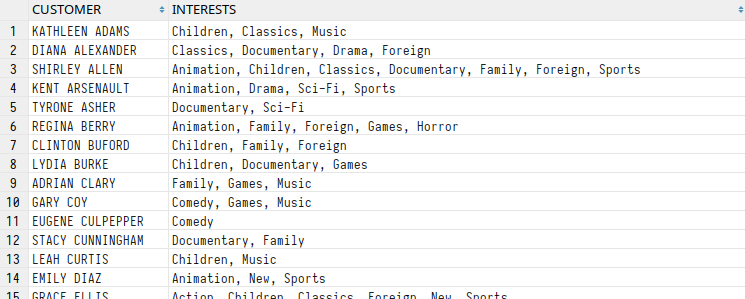
\includegraphics[width=\textwidth]{images/1_3.png}
		\caption{Resultat der Abfrage 1.3}
	\end{figure}

	%2.1
	\begin{figure}[H]\centering
		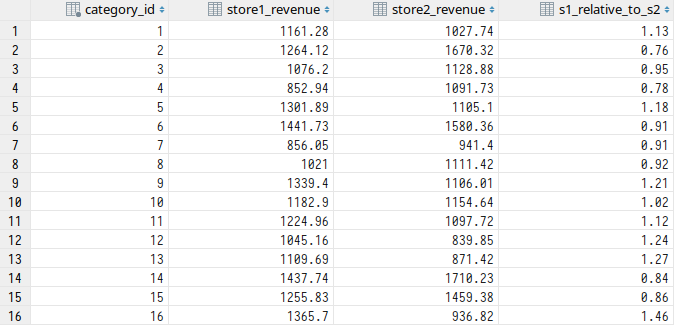
\includegraphics[width=\textwidth]{images/2_1.png}
		\caption{Resultat der Abfrage 2.1}
	\end{figure}

	%3.1
	\begin{figure}[H]\centering
		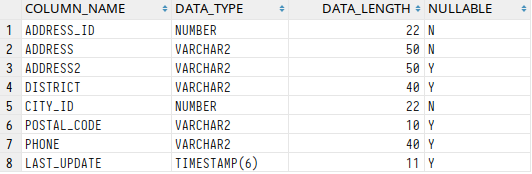
\includegraphics[width=\textwidth]{images/3_1.png}
		\caption{Resultat der Abfrage 3.1}
	\end{figure}

	%3.2
	\begin{figure}[H]\centering
		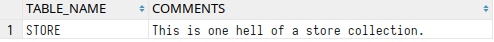
\includegraphics[width=\textwidth]{images/3_2.png}
		\caption{Resultat der Abfrage 3.2}
	\end{figure}

	%3.3
	\begin{figure}[H]\centering
		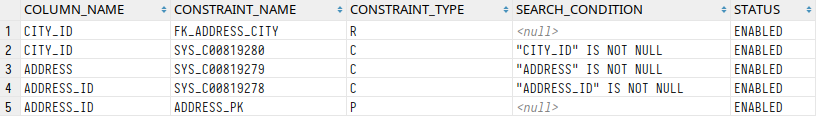
\includegraphics[width=\textwidth]{images/3_3.png}
		\caption{Resultat der Abfrage 3.3}
	\end{figure}

	%4.1
	\begin{figure}[H]\centering
		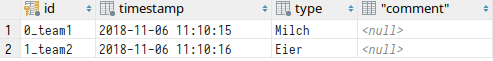
\includegraphics[width=\textwidth]{images/4_1.png}
		\caption{Resultat der Abfrage 4.1}
	\end{figure}

	\section*{Theorie}
	\subsection*{4.2 Autokennzeichen}
		Autokennzeichen sind künstliche Schlüssel, die sich aus verschiedenen
		Informationen zusammensetzen, wie zum Beispiel dem Sitz der Behörde, bei der
		ein besimmtes Auto angemeldet ist. Es eignet sich nicht als Primärschlüssel 
		für Kunden, da man mehrere Autos auf seinen Namen anmelden kann und deswegen 
		Kunden der Autostatt zwei mal aufgeführt wären. Weiters ist das Kennzeichen
		ungeeignet als Primärschlüssel für Auto-Relationen, da bei einem Umzug das
		Auto (Modell, Zustand etc.) gleich bleibt, sich die Kenntafel aber ändert.
		
	\subsection*{4.3 ISBN}
		Die ISBN ist eine Kombination von Nummern, welche Informationen über Titel,
		Verlag etc. geben, sie ist demnach ein zusammengesetzter / künstlicher Schlüssel.
		Sie identifiziert ein Buch und kein Exemplar eines Buches und ist deshalb
		ungeeignet als (einziger) Primärschlüssel für Buchexemplare, da eine Bibliothek 
		ohne weiteres mehrere Exemplare eines Buches im Bestand haben kann. Wird der ISBN 
		aber als Schlüssel für Bücher (nicht Exemplare) verwendet, ist das kein Problem - 
		schlie{\ss}lich ist das der Sinn einer ISBN.
\end{document}